\begin{answer}
\begin{figure}[H]
  \centering
  \vspace{-2mm}
  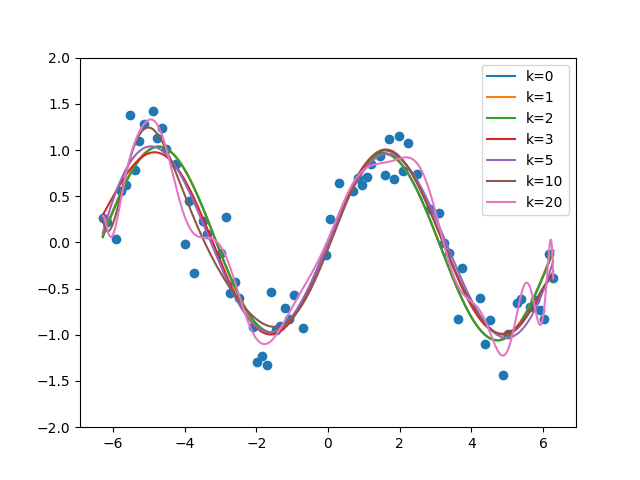
\includegraphics[width=0.65\linewidth]{../src/featuremaps/large-sine.png}
  \centering
\caption{Polynomial regression with other features with kernel sizes 0,1,2,3,5,10 and 20}
\end{figure}

In the presence of the sin($x$) feature, the models seem to fit the data better / more robustly. However the numerical instability that comes with high degree polynomials remain.

\end{answer}
